\begin{sidewaystable}
%\begin{table}[h]
\caption{Building up the response function $Y(b)$: the amplitudes $c$ in equation \eqref{eq:upsilon}.}
\begin{center}
\begin{tabular}{cccc}
 %
   order & fit vs. ideal & residual error & monomial amplitudes $c_{2k}$ \\[10pt]
 %
   $10$ &
   \raisebox{-0.5\height}{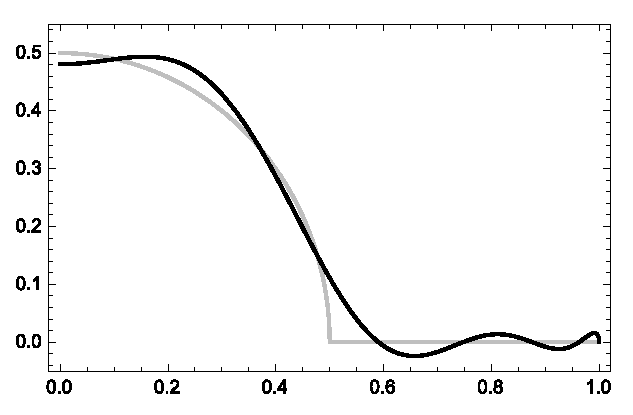
\includegraphics[ width = 2.25in ]{graphics/new_fit_10.eps}} &
   \raisebox{-0.5\height}{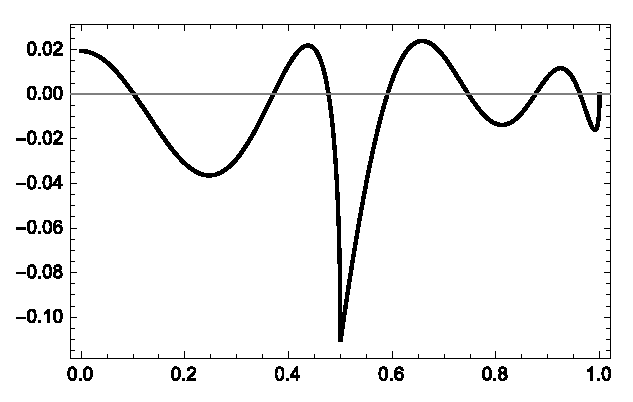
\includegraphics[ width = 2.25in ]{graphics/new_residual_error_10.eps}} &
   \raisebox{-0.5\height}{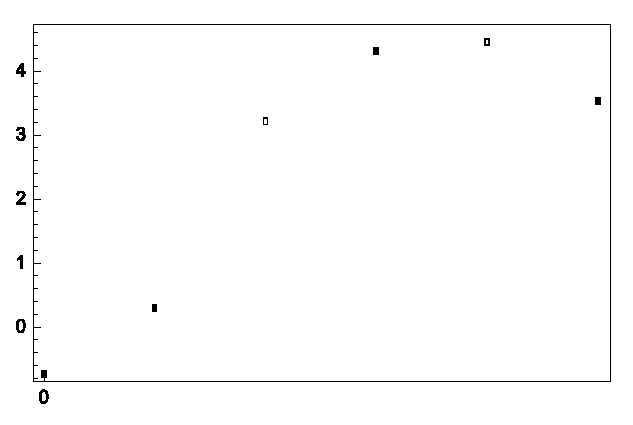
\includegraphics[ width = 2.25in ]{graphics/new_checkers_10.eps}} \\[15pt]
 %
   $100$ &
   \raisebox{-0.5\height}{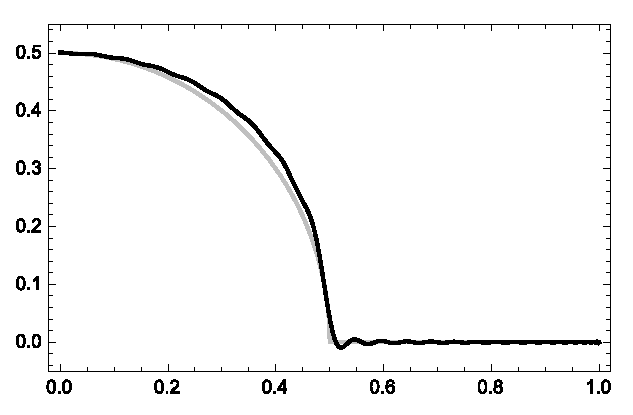
\includegraphics[ width = 2.25in ]{graphics/new_fit_100.eps}} &
   \raisebox{-0.5\height}{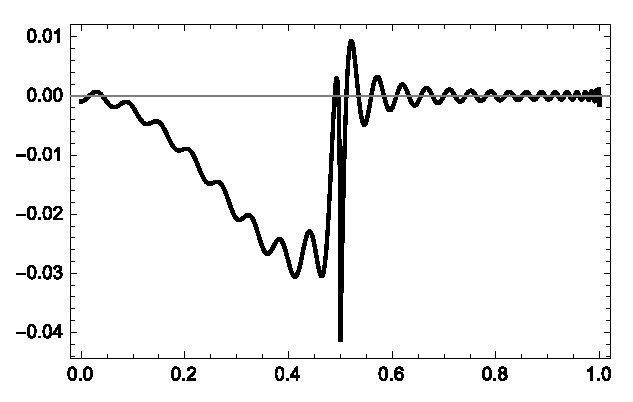
\includegraphics[ width = 2.25in ]{graphics/new_residual_error_100.eps}} &
   \raisebox{-0.5\height}{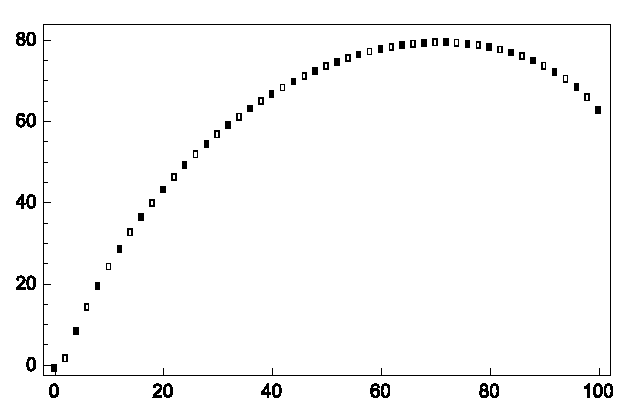
\includegraphics[ width = 2.25in ]{graphics/new_checkers_100.eps}} \\[15pt]
 %
   $200$ &
   \raisebox{-0.5\height}{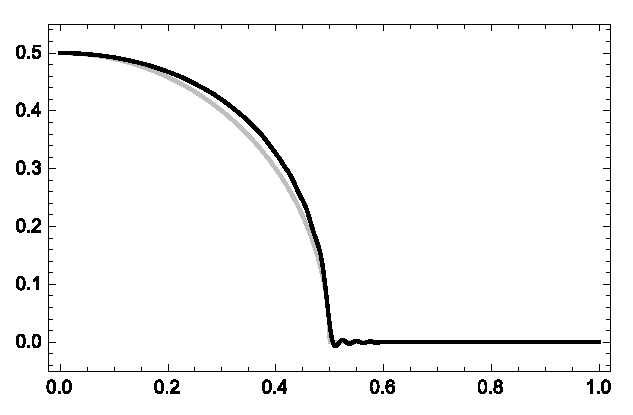
\includegraphics[ width = 2.25in ]{graphics/new_fit_200.eps}} &
   \raisebox{-0.5\height}{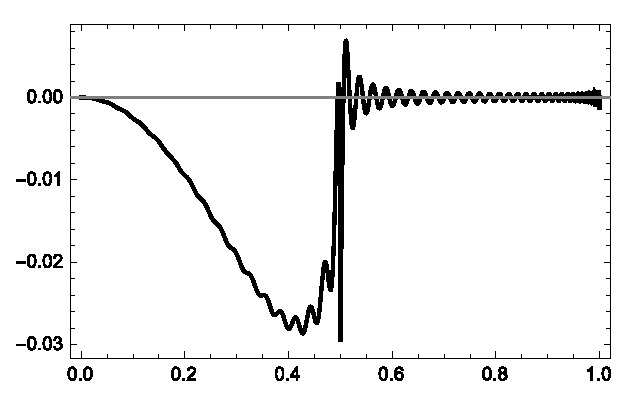
\includegraphics[ width = 2.25in ]{graphics/new_residual_error_200.eps}} &
   \raisebox{-0.5\height}{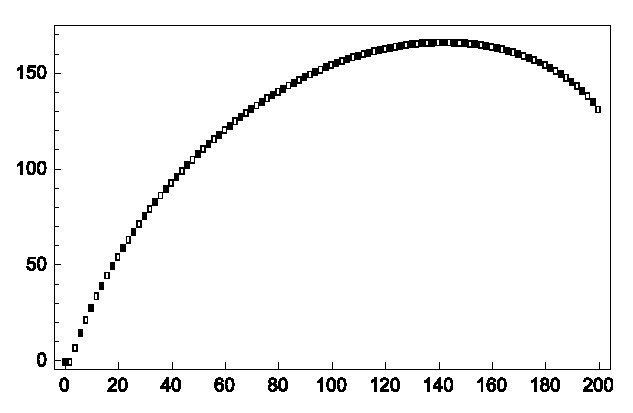
\includegraphics[ width = 2.25in ]{graphics/new_checkers_200.eps}} \\
 %
 %
 %
\end{tabular}
\end{center}
\label{tab:response function fit}
%\end{table}

\end{sidewaystable}

\endinput %-------------------------------